\documentclass[]{article}
\usepackage{graphicx}

%opening
\title{TDDD41 - Lab 1}
\author{}

\begin{document}

\maketitle

\section{Simple k-means}

\textbf{1. Choose a set of attributes for clustering and give a motivation. (Hint: always ignore attribute "name". Why does the name attribute need to be ignored?)}
The \textit{name} attribute is basically metadata, in the sense that it does not carry meaning during a data analysis and is only used to label the data points. For what concerns the choice of attributes, we tried to choose attributes that do not seem to be directly correlated. For instance, we picked protein and fat over energy, because energy in meat is largely depending on those two attributes, and it could make the analysis more complex without providing a lot of extra information. Then we chose to pick calcium.\\

\noindent\textbf{2. Experiment with at least two different numbers of clusters, e.g. 2 and 5, but with the same seed value 10.}
The more clusters we have, the more specific subdivisions we get. Because of the nature of k-means, that is partitioning and non-overlapping, it might not carry a lot of significance to cluster data in very small sets. Mostly the $k$ parameter should be tuned according to which information we are looking for. We experimented with $k=2,3,8$.\\

\noindent\textbf{3. Then try with a different seed value, i.e. different initial cluster centers. Compare the results with the previous results. Explain what the seed value controls.}
The seed value controls the starting points of the cluster centroids. If we change the value of the seed, the algorithm seems much more unstable for larger values of $k$, producing quite different clusters, which is likely also due to the fact that we have such a small dataset. However, if $k$ is small, the clusters produced are quite similar for different seeds. With $k=2$ and $k=3$, for instance, the results are quite similar, evaluating by the centroids of the clusters. For $k=8$, much less so. We chose these values in order to compare how meaningful the clusters when there are many vs when there are few. The number of data points in the clusters may vary too with the seed. This, along with the fact that the algorithms converges after many less iterations that the maximum we supply of 500, shows that k-means does not generate solutions corresponding to the global optimum, because otherwise starting by only changing the seed values would result in the same solutions. Instead, local optima are reached and then the algorithm stops. The choice of the seed values is somewhat arbitrary as they just influence a random starting point.\\

\noindent\textbf{4. Do you think the clusters are "good" clusters? (Are all of its members "similar" to each other? Are members from different clusters dissimilar?)}
As we mentioned in question 2., how good our clusters are essentially depends on what attibutes we are looking at. Since there are many variables, it is hard to visualize them at once, so a useful way is to visualize each variable against itself to see if similar elements get into similar clusters. In the plots below we can see that elements of a single cluster tend to be quite similar among each other in terms of fat and calcium---while they are dissimilar to members of the other cluster---, but dissimilar in terms of protein content---and conversely tend to be similar to members of another cluster.\\

\includegraphics[scale=0.65]{figures/calcium_calcium.eps}

\noindent Figure 1: The blue cluster has very low levels of calcium, the red cluster covers all other amounts. There seems to be little overlap.


\includegraphics[scale=0.65]{figures/fat_fat.eps}

\noindent Figure 2: The blue cluster has higher amounts of fat, the red cluster has smaller amounts. Within-cluster elements have high similarity.

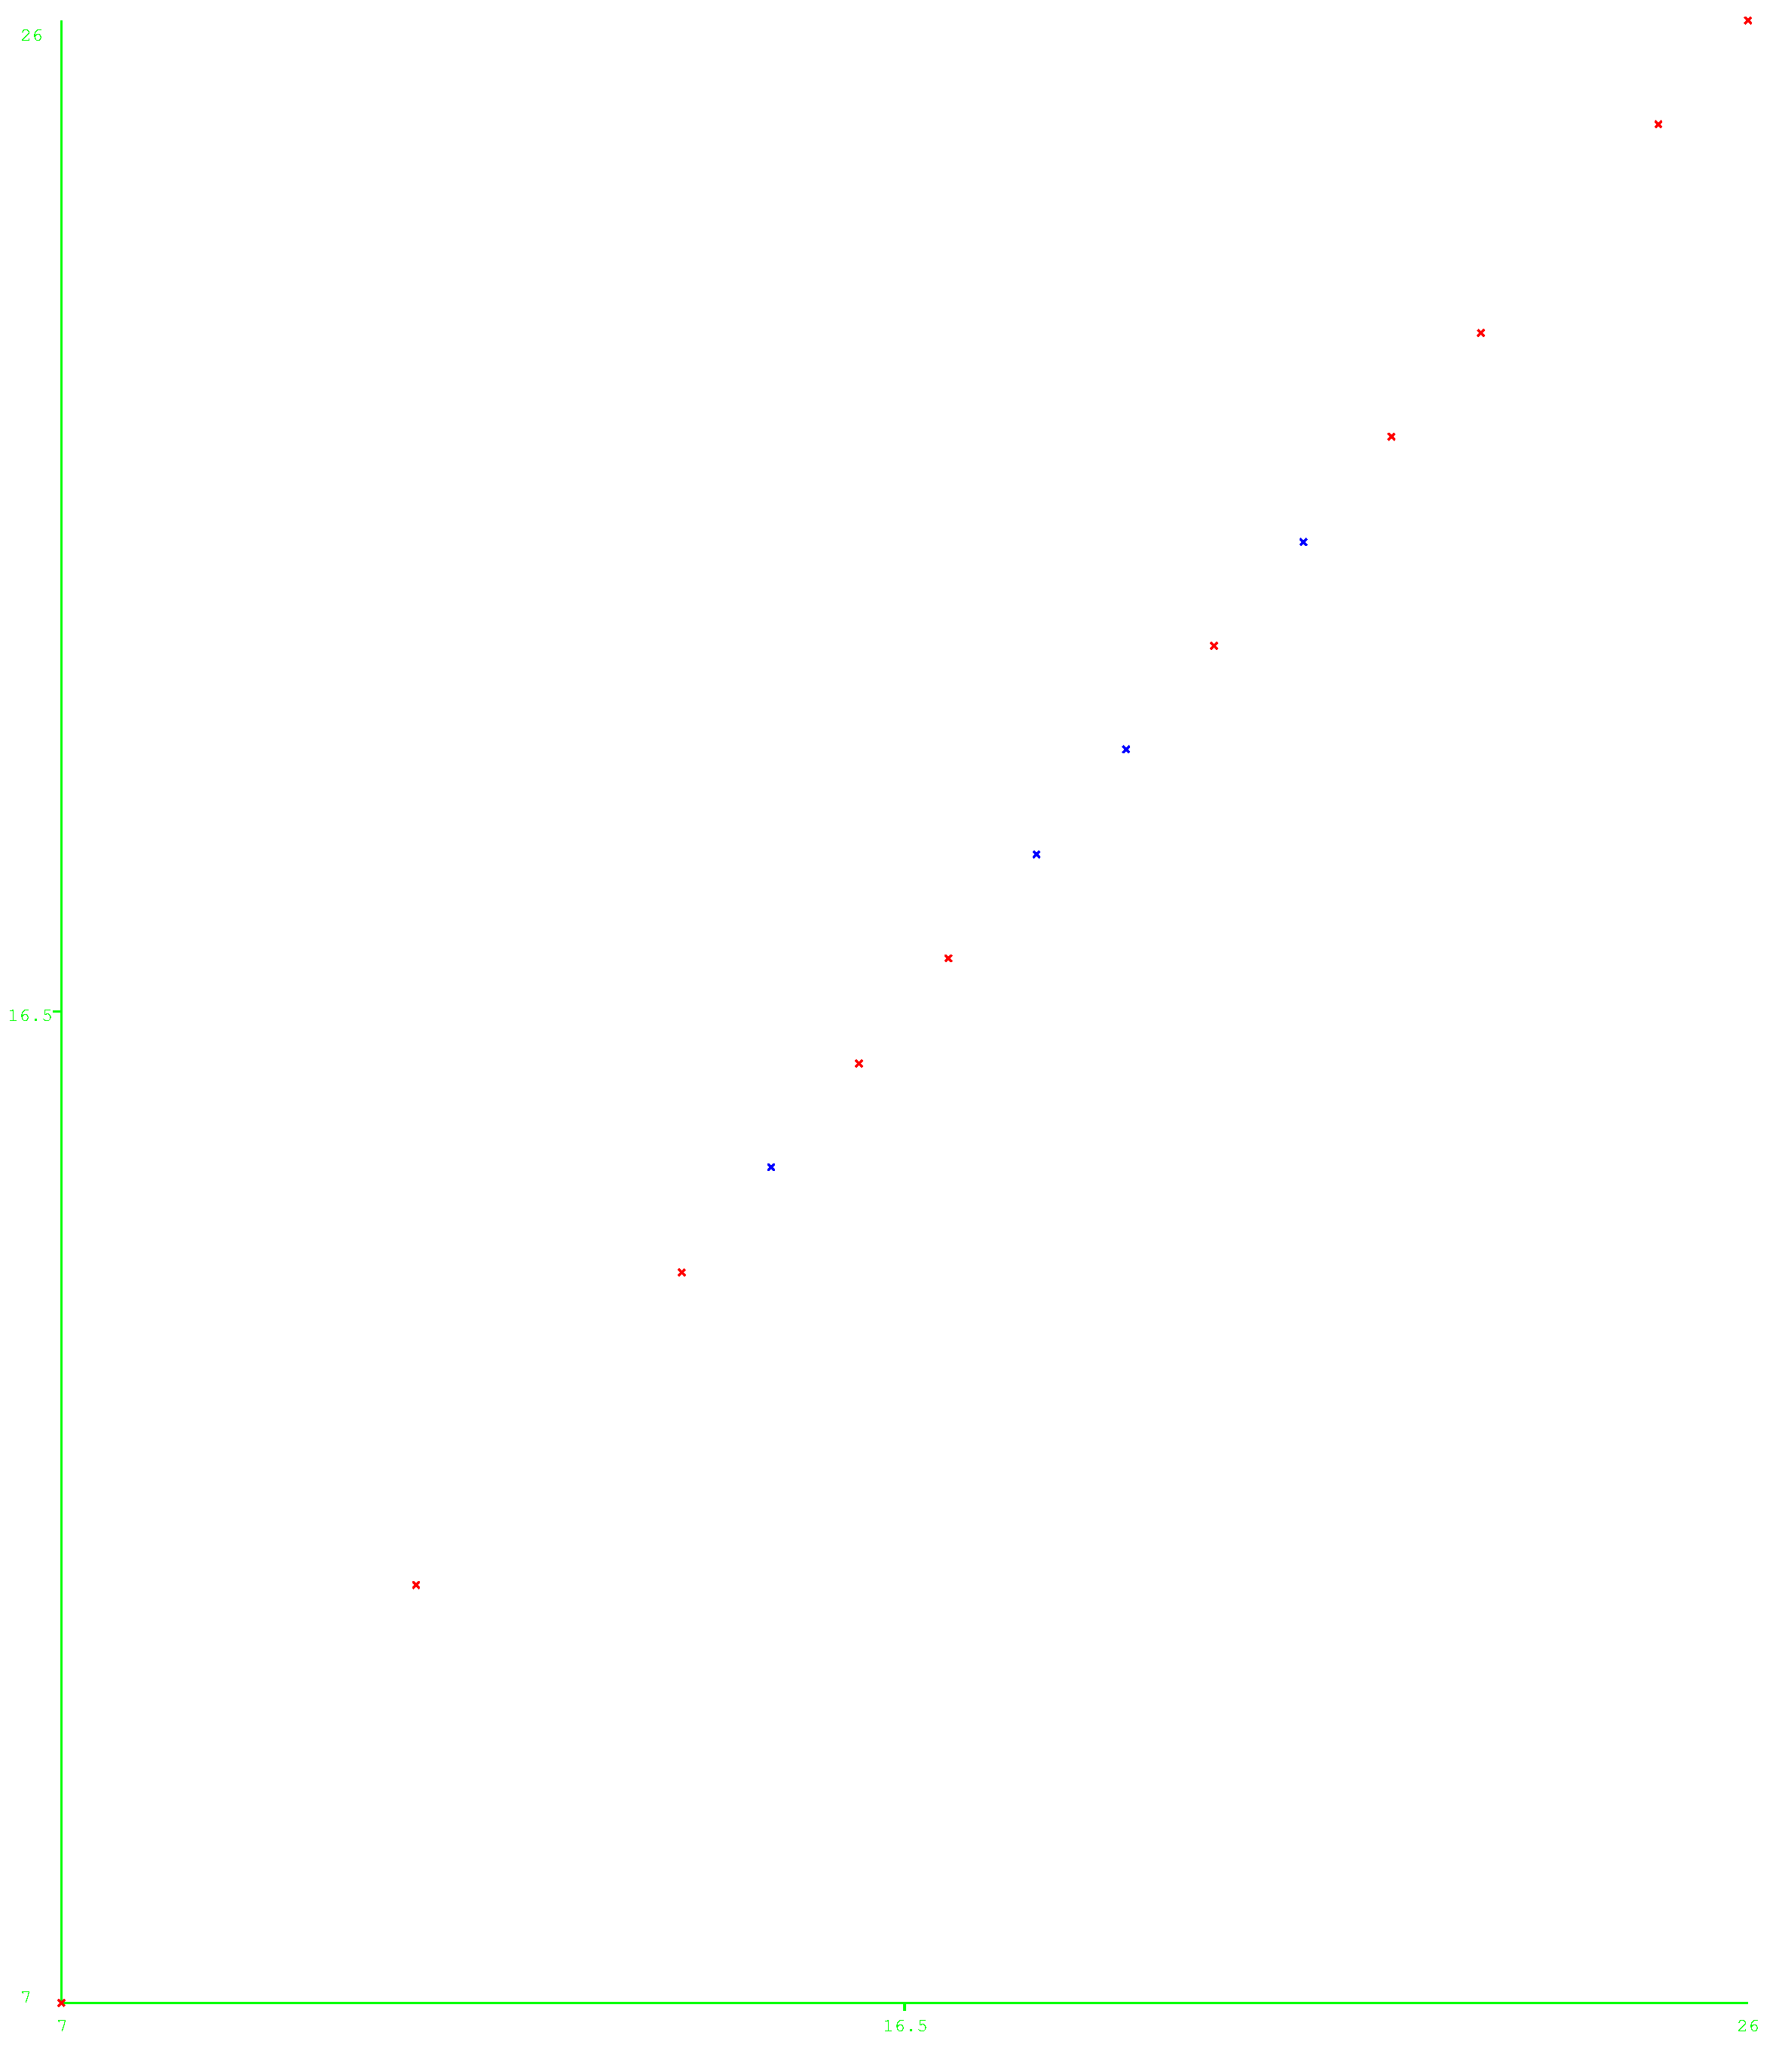
\includegraphics[scale=0.25]{figures/protein_protein.eps}

\noindent Figure 3: The clustering is not good w.r.t. protein. We see that the two clusters overlap in terms of protein content, and within-cluster similarity is low.\\

\noindent\textbf{5. What does each cluster represent? Choose one of the results. Make up labels (words or phrases in English) which characterize each cluster.}
We chose $k=2$ with seed 10. As can be seen in the plots above, the clearest separation is in terms of fat content. In particular, we can see that very fatty foods contain very little calcium. The blue cluster contains meats that are high in fat and contain very little calcium, while the red cluster contains meats that are low in fat.

% Messy stuff below, needs to be tidied

\section{MakeDensityBasedClusters}
\textbf{2. Experiment with at least two different standard deviations. Compare the results. (Hint: Increasing the standard deviation to higher values will make the differences in different runs more obvious and thus it will be easier to conclude what the parameter does).} 
The standard deviation parameter influences the size of the final clusters. First, the algorithm produces clusters according to k-means, and then adjusts them with the minimum standard deviation. If we have a sufficiently small minimum standard deviation, we are guaranteed that we will have as many clusters as we originally asked for, in our case $k=2$. However, if the standard deviation is too large we will end up including points that are dissimilar among each other, or even reducing the number of clusters, as more and more points need to be included to satisfy the deviation requirement, and they have to be taken from other clusters. If the standard deviation for an attribute within a cluster is large relative to the deviations for the other attributes, that means that the attribute does not contribute particularly much to characterizing the cluster. Then, if the means for the same attribute in different clusters are very different, we also have to take a look at the respective standard deviations in order to know if this difference is significant to our clustering or not. For instance, with $k=2$ we used first the default minimum of $\sigma=1.0E-6$, and we ended up with two clusters, and then did the same for $\sigma=10$, which also gave two clusters, even if one of them takes two elements from the other cluster in order to increase its deviation. With $\sigma=1000$, all elements end up being in one cluster.


\end{document}
